\addcontentsline{toc}{section}{Introduction}
\section*{Introduction}
Ce chapitre s'attelle à la présentation du prototype de StudX, l’application de communication en temps réel que nous proposons. 
Nous en présenterons les diverses fonctionnalités accompagnées de capture d'écran. 
Puis, au travers d’une discussion, nous en présenterons les limites, les contraintes et les possibilités d’expansion.

\section{Résultats}
\subsection{Authentification}
L'accès à l’application est subordonné à l'authentification de l’utilisateur. 
La figure \ref{fig:proto_auth} en présente l’interface. 
Elle offre la possibilité de se connecter ou de s'inscrire.

\begin{figure}[h]
  \centering
  \frame{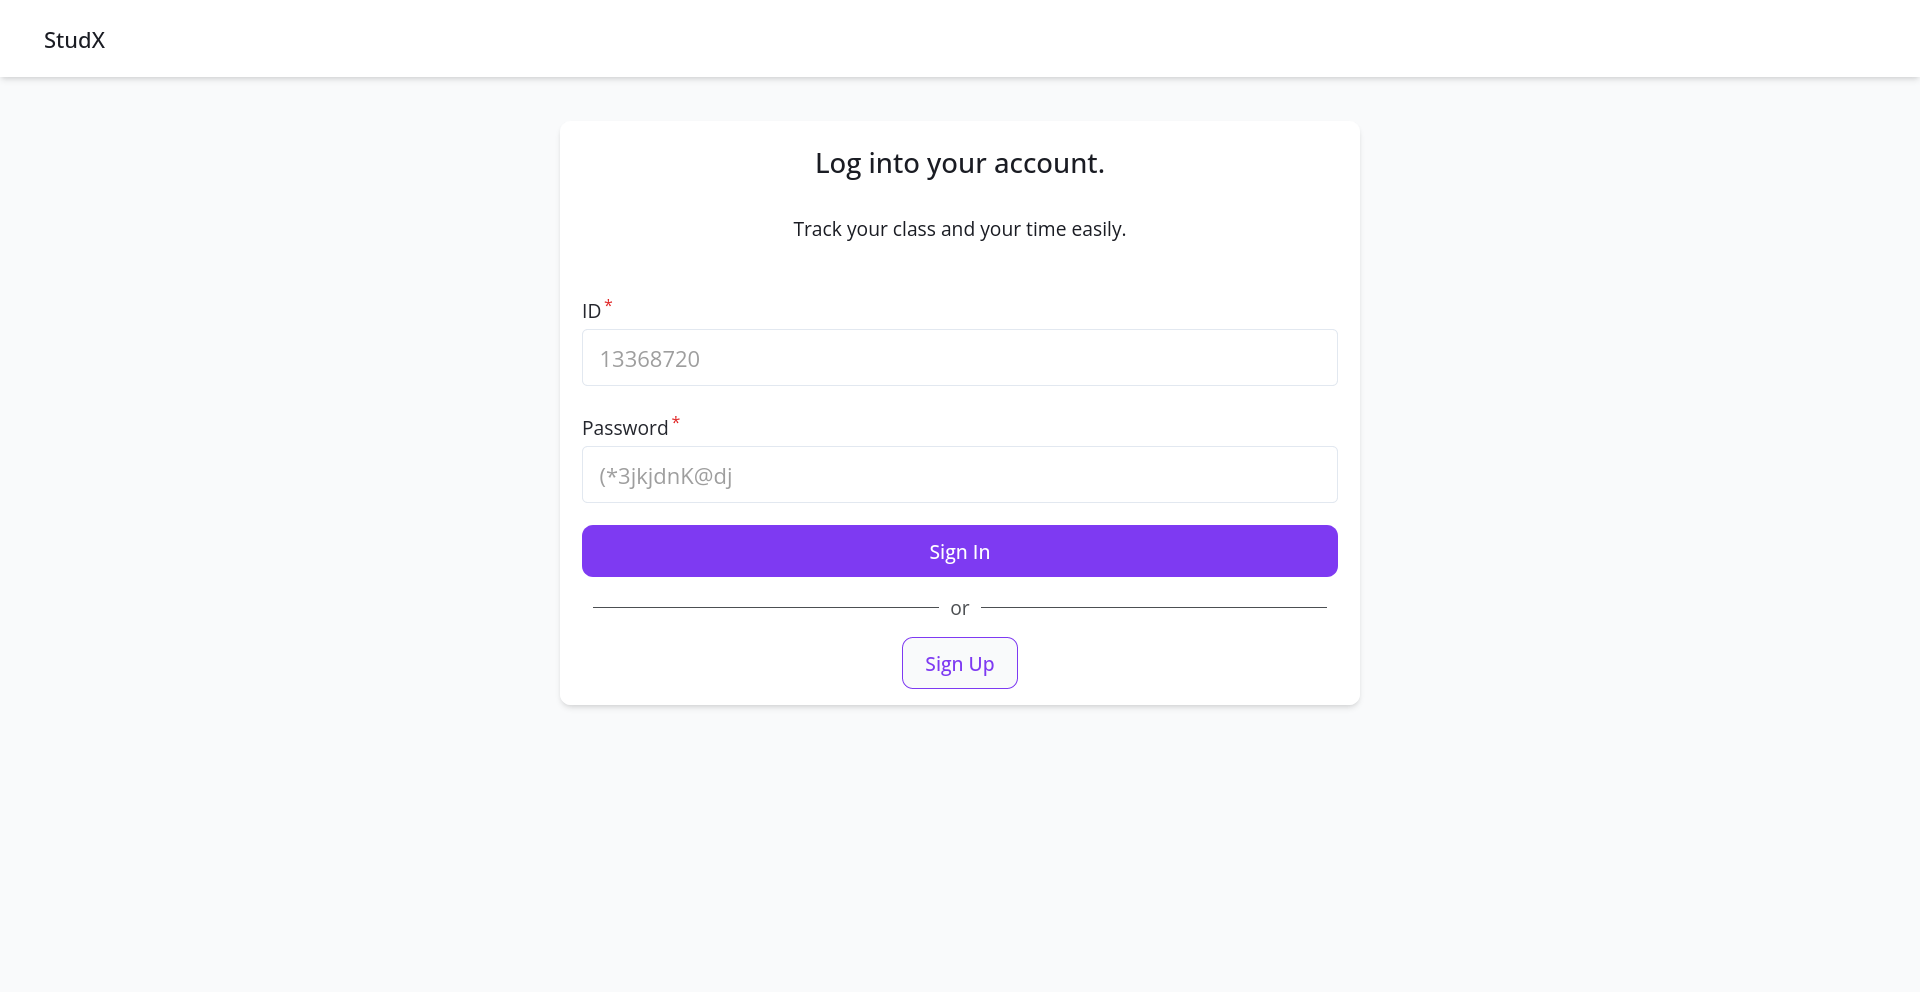
\includegraphics[width=0.85\textwidth]{prototype/login}}
  \caption{Page d'authentification de \textbf{StudX}}
  \label{fig:proto_auth}
\end{figure}

\subsection{Calendrier}
Après authentification, l’utilisateur accède au calendrier des divers événements planifiés. 
Il lui est possible de réduire ou d'étendre la vue au jour actuel, aux semaines ou encore aux mois.  
S’il s’agit d’un administrateur ou d’un enseignant, il peut en ajouter de nouveaux.
La figure \ref{fig:proto_calendar_view} présente le calendrier,qui présente tous les programmes du mois courant.

\begin{figure}[h]
  \centering
  \frame{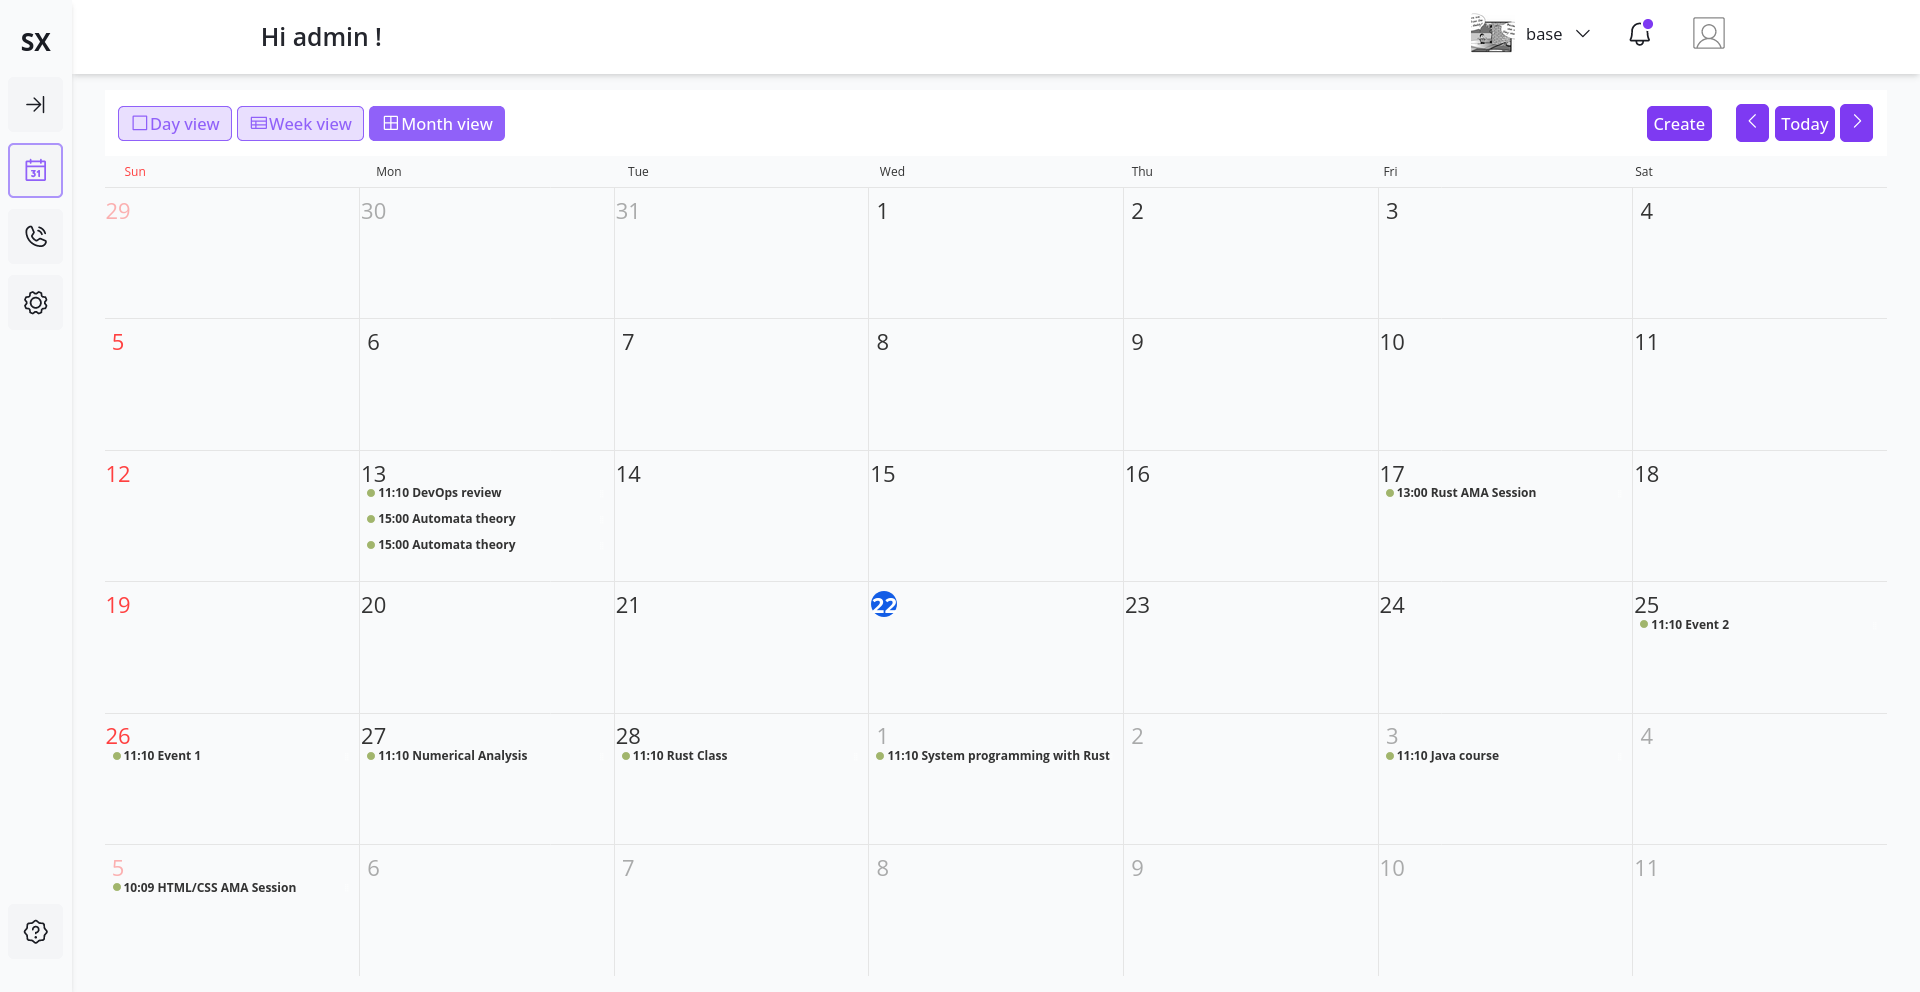
\includegraphics[width=0.85\textwidth]{prototype/calendar-view}}
  \caption{Calendrier des planifications}
  \label{fig:proto_calendar_view}
\end{figure}

S’il dispose des permissions nécessaires, 
l’utilisateur peut ajouter un événement au calendrier en suivant le formulaire que montre la figure \ref{fig:add_event}.


\begin{figure}[h]
  \centering
  \frame{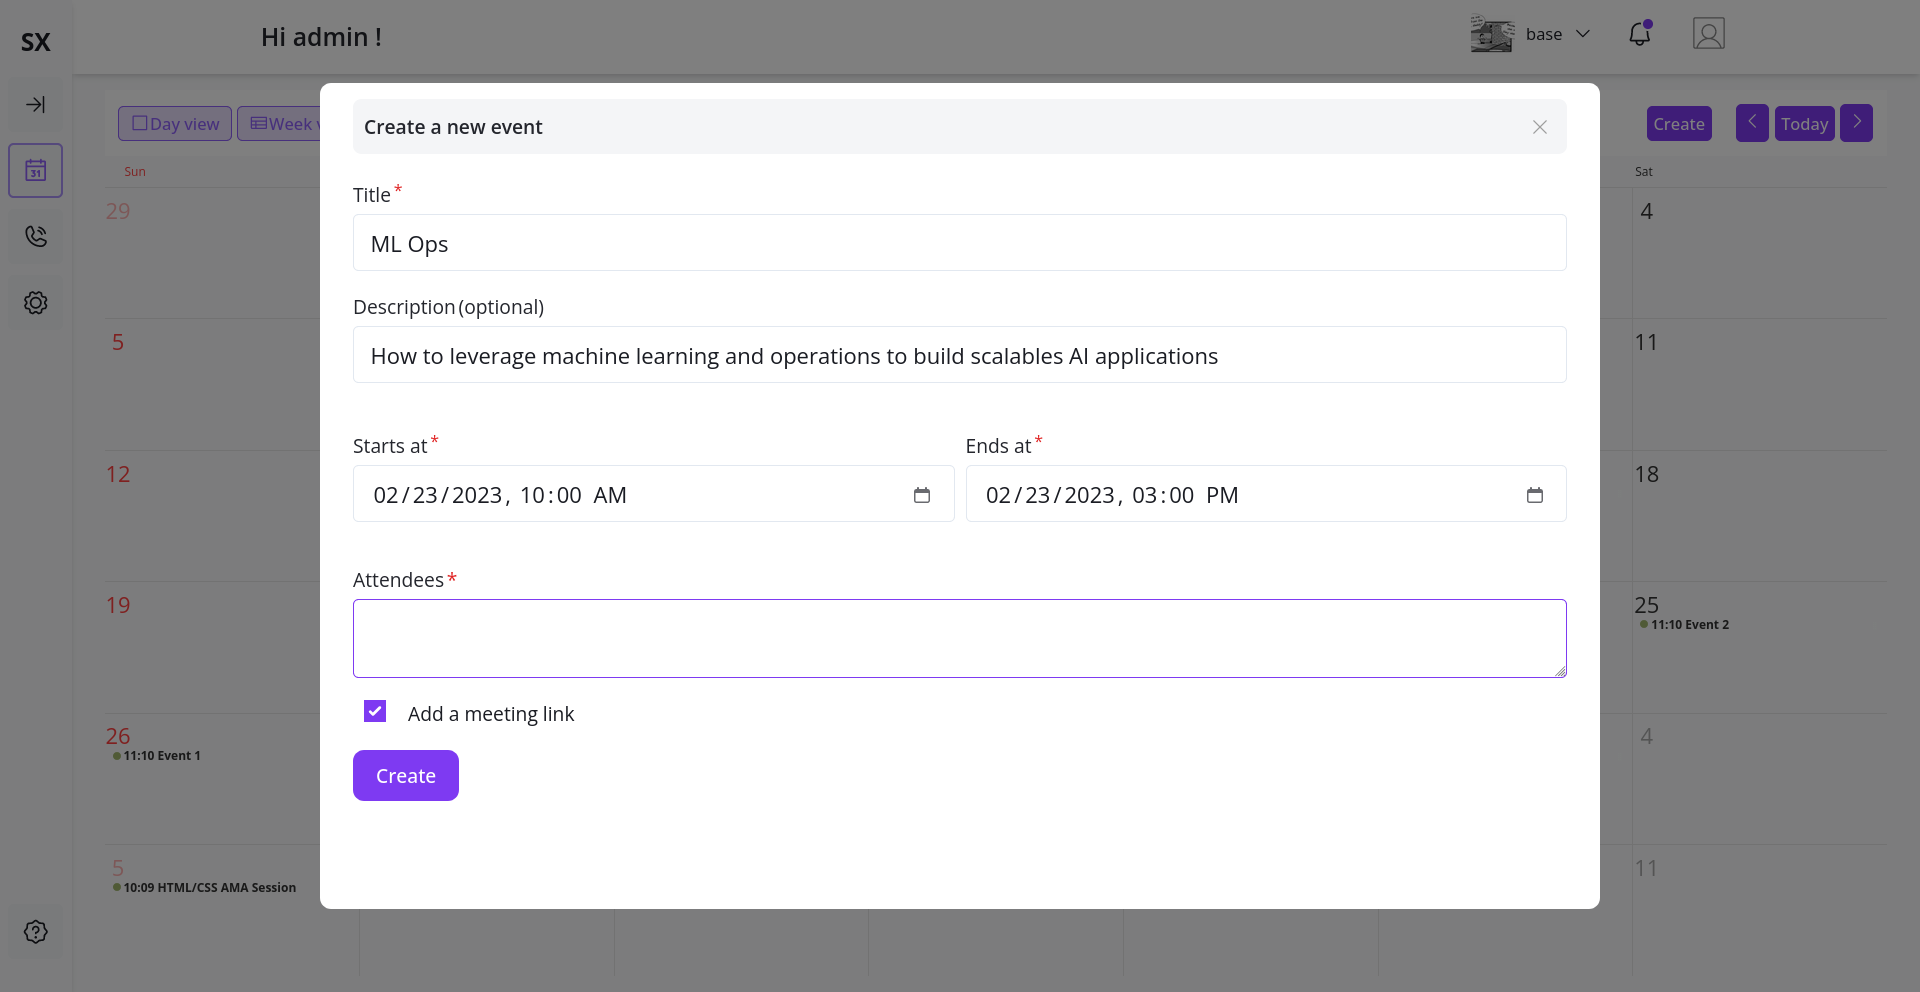
\includegraphics[width=0.85\textwidth]{prototype/add-event-form}}
  \caption{Calendrier des planifications}
  \label{fig:add_event}
\end{figure}

Il est possible d’associer à l'événement un lien d'accès à la session de conférence en ligne. 
Pour y accéder par la suite, les utilisateurs peuvent consulter les détails dudit événement (figure \ref{fig:event_details}).

\begin{figure}[h]
  \centering
  \frame{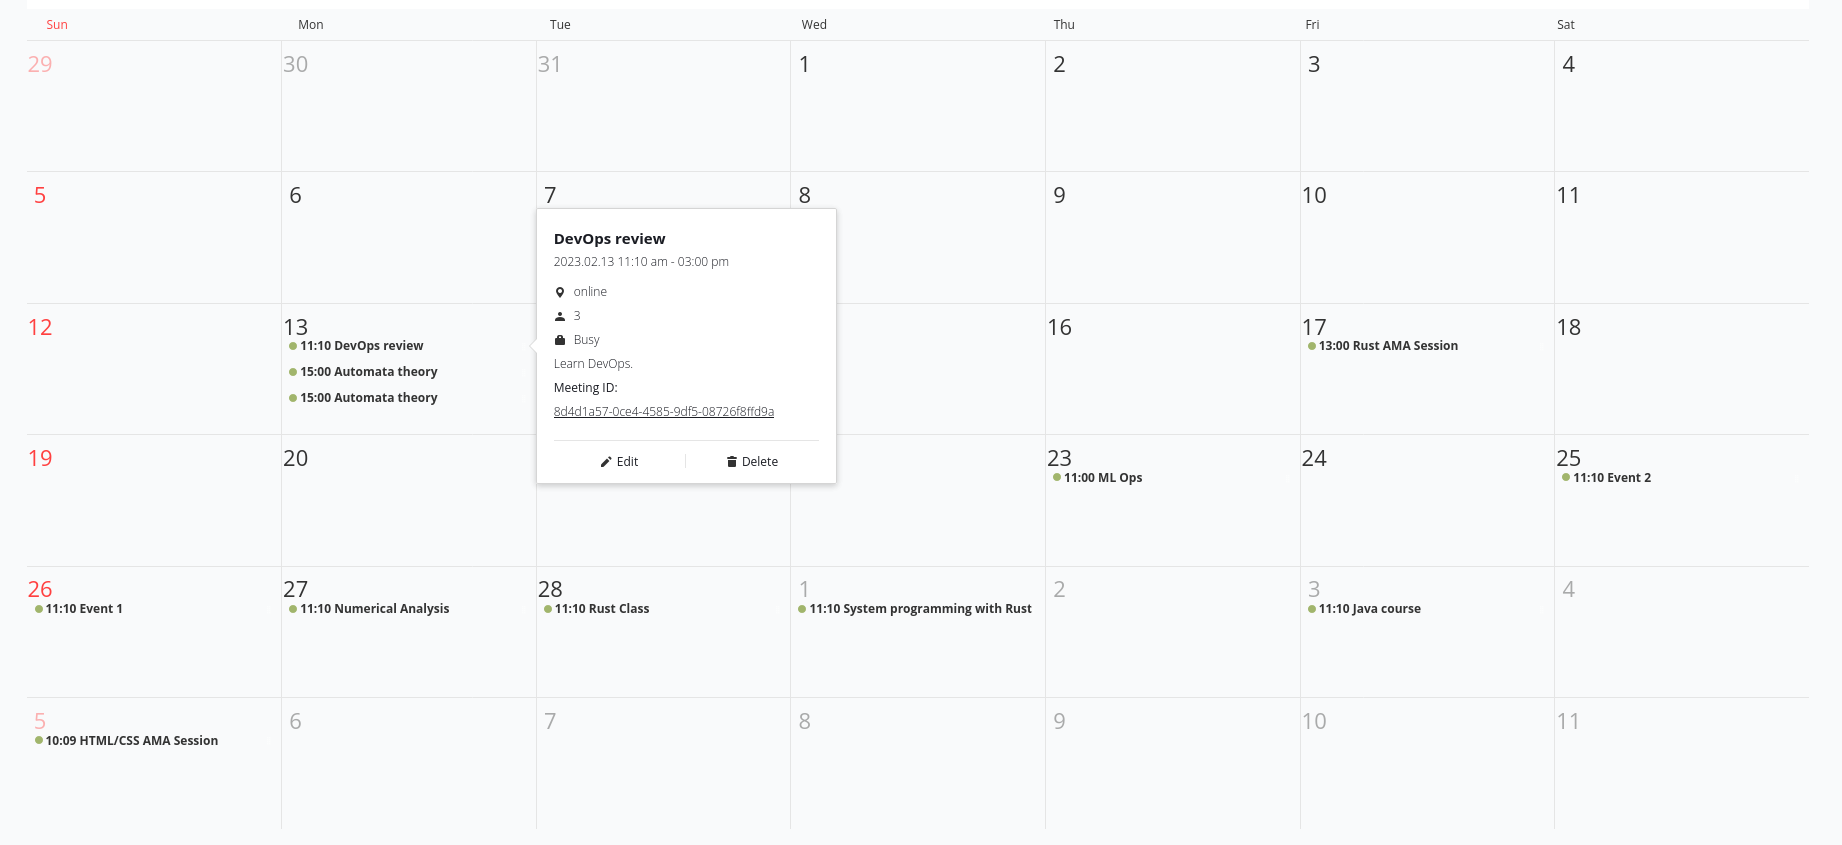
\includegraphics[width=0.85\textwidth]{prototype/event-detail}}
  \caption{Détails d'un événement}
  \label{fig:event_details}
\end{figure}

\subsection{Sessions en ligne}
Les événements incluant un lien donnent accès à une session en ligne que
peuvent rejoindre tous les participants disposant du lien.

Les figures \ref{fig:single_user} et \ref{fig:many_users} présentent à quoi ressemble l’interface par défaut. 
Elles présentent, en fait, la grille des participants et l’interface de contrôle.


\begin{figure}[h]
  \centering
  \frame{
\includegraphics[width=0.85\textwidth]{prototype/user-single-in-room}}
  \caption{Grille des participants avec un seul participant présent}
  \label{fig:single_user}
\end{figure}


\begin{figure}[h]
  \centering
  \frame{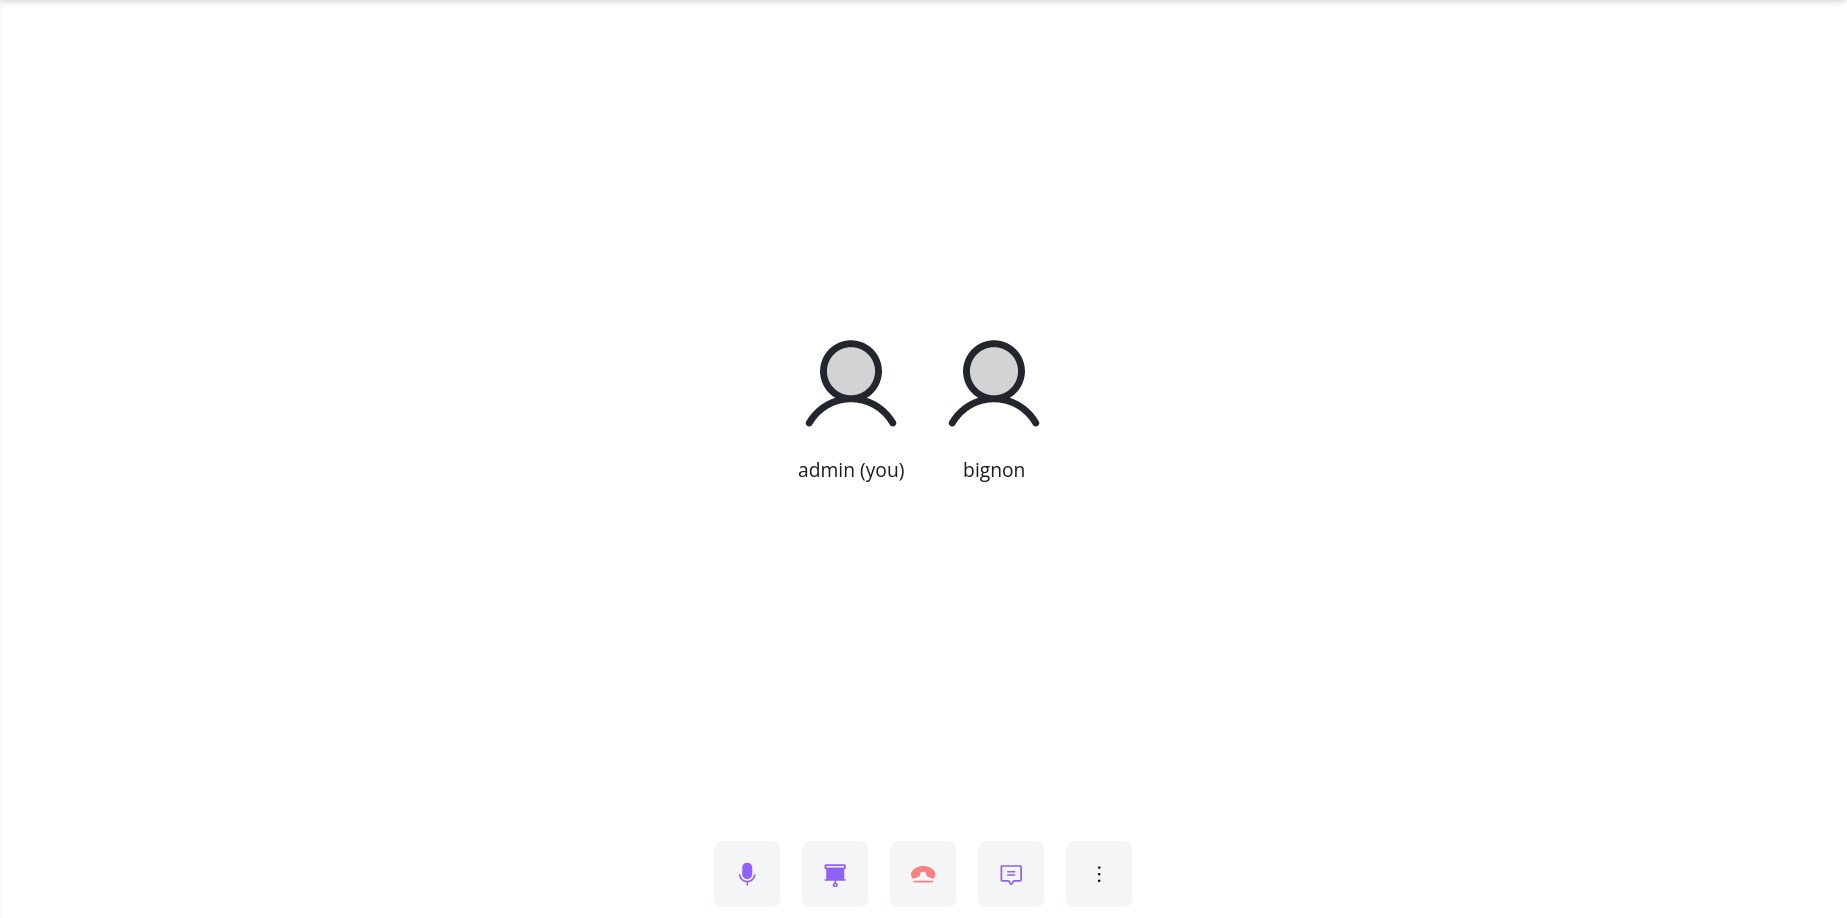
\includegraphics[width=0.85\textwidth]{prototype/user-with-participants-in-room}}
  \caption{Grille des participants avec plus d'un utilisateur}
  \label{fig:many_users}
\end{figure}

\newpage
Outre la voix, les participants ont la possibilité d’interagir entre eux via des messages écrits (figure \ref{fig:room_chat}).

\begin{figure}[h]
  \centering
  \frame{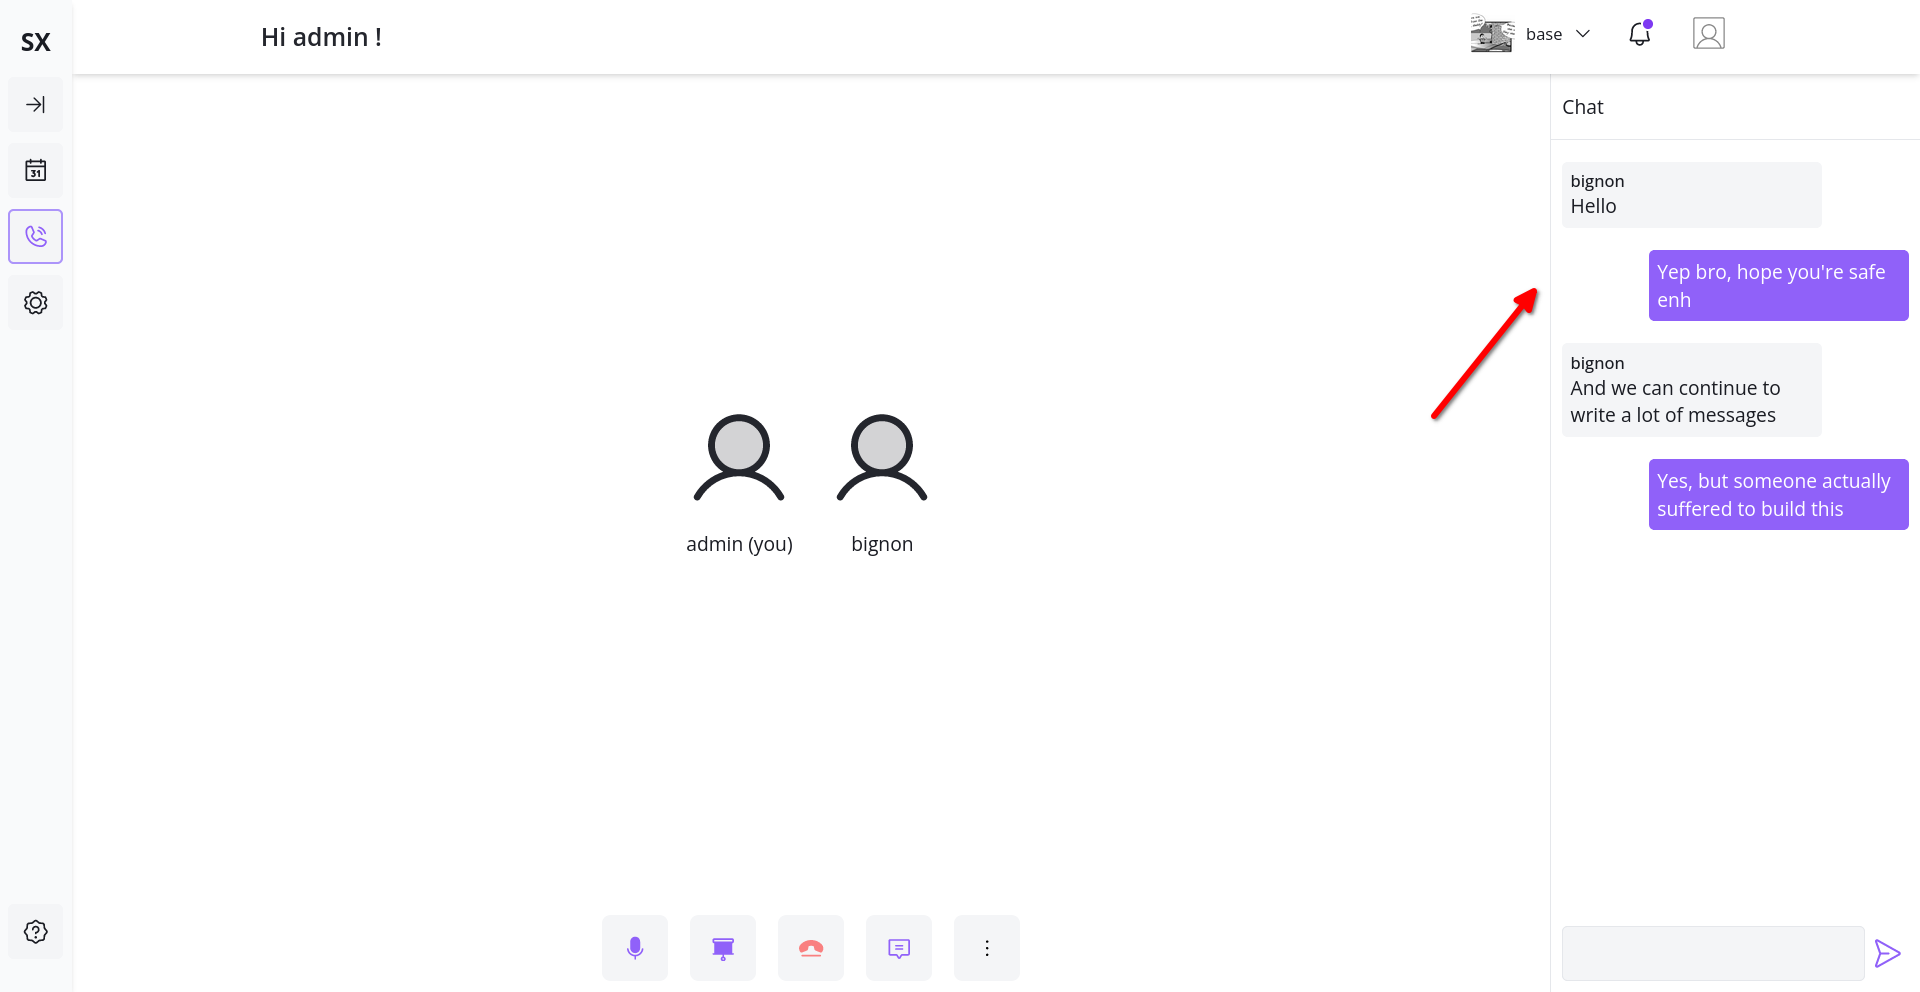
\includegraphics[width=0.85\textwidth]{prototype/room-chat}}
  \caption{Messagerie instantannée intégrée à \textbf{StudX}}
  \label{fig:room_chat}
\end{figure}

Plusieurs autres fonctionnalités sont exploitables. 
L’une d’elles est le partage d'écran. Pour illustrer, nous nous sommes servis de deux appareils avec 
l’un faisant le partage, comme le montre les figures \ref{fig:sharing_screen} et \ref{fig:viewing_screen}.

\newpage
\begin{figure}[h]
  \centering
  \frame{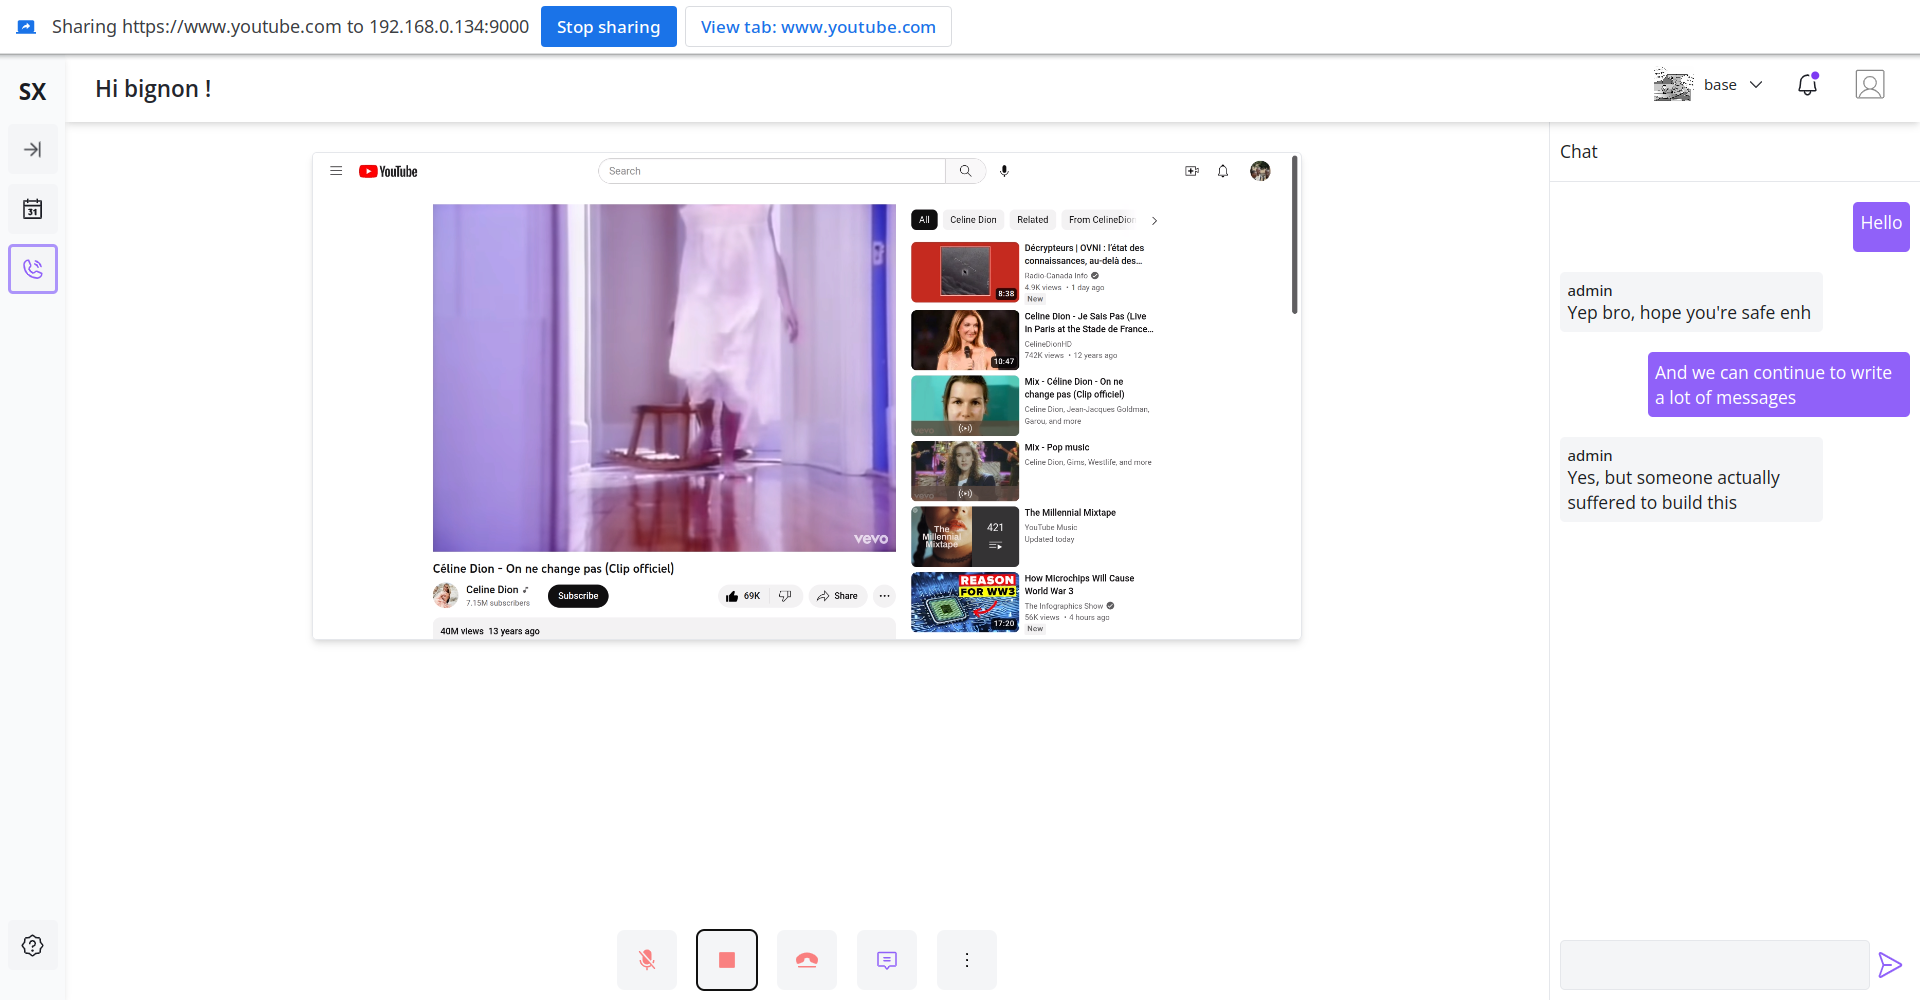
\includegraphics[width=0.85\textwidth]{prototype/user-sharing-screen}}
  \caption{Partage d'écran}
  \label{fig:sharing_screen}
\end{figure}

\newpage
\begin{figure}[h]
  \centering
  \frame{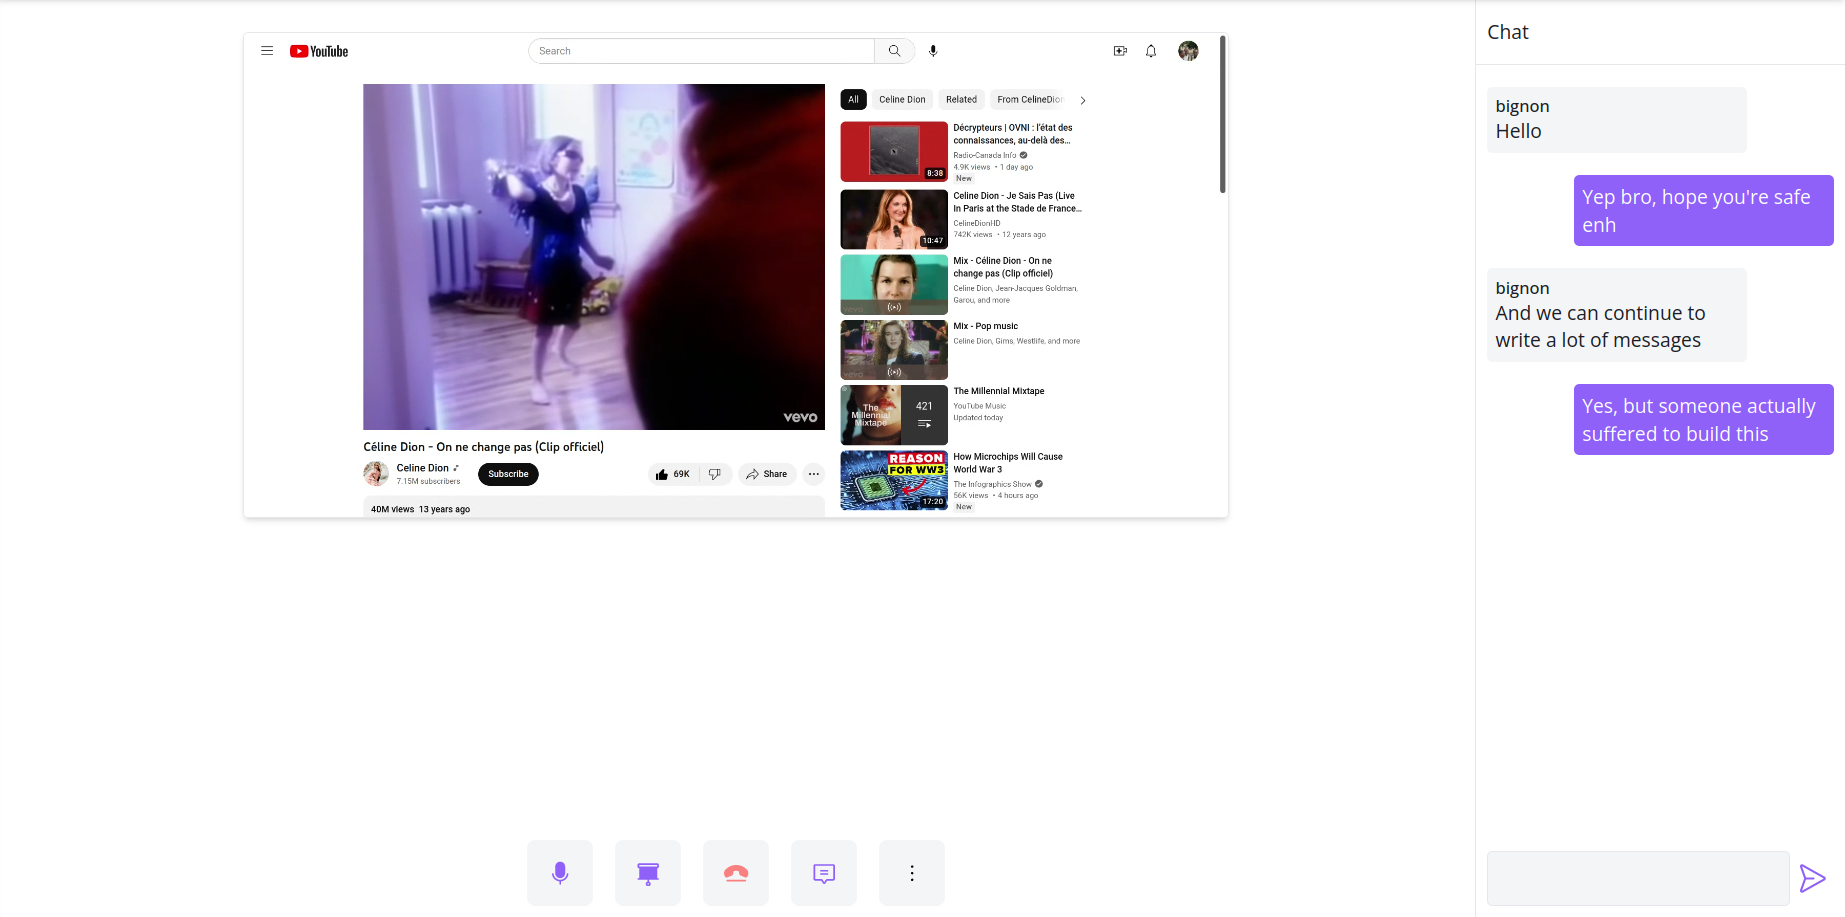
\includegraphics[width=0.85\textwidth]{prototype/user-viewing-screen}}
  \caption{Visualisation de l'écran partagé}
  \label{fig:viewing_screen}
\end{figure}

Les participants disposent également d’un whiteboard, 
c'est-à- dire un tableau virtuel, pour effectuer des illustrations. 
Le contenu est synchronisé entre tous les participants. 
La figure 3.10 fait une démonstration de ladite fonction.

\begin{figure}[h]
  \centering
  \frame{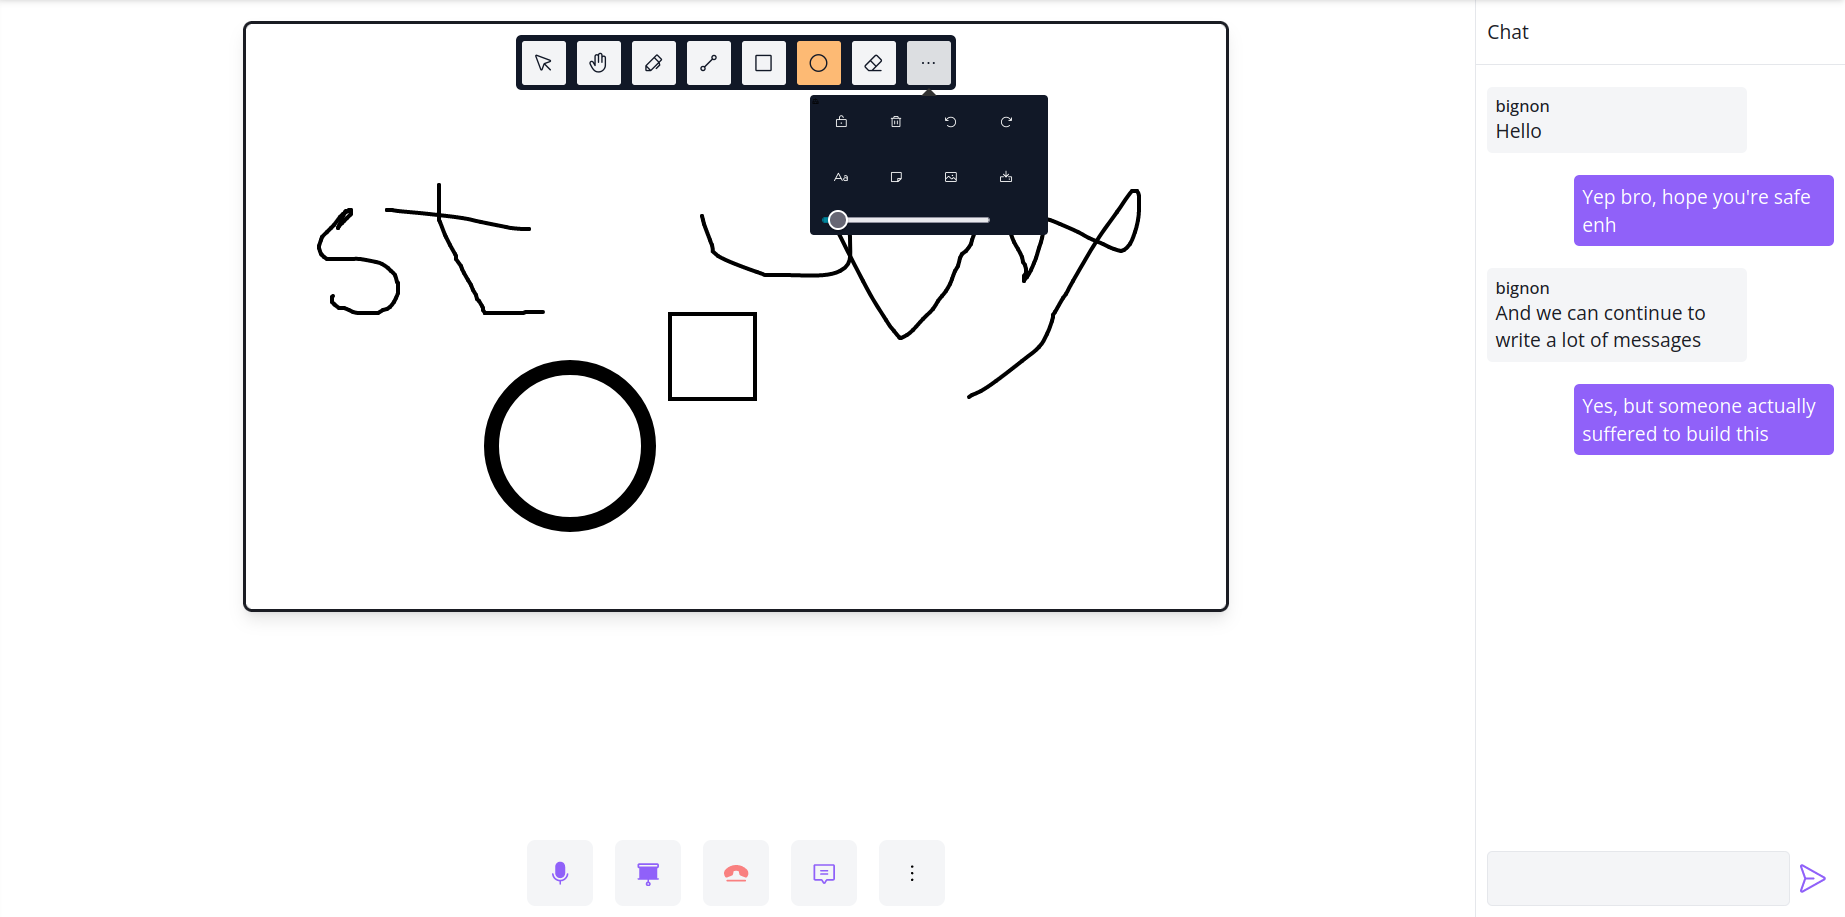
\includegraphics[width=0.85\textwidth]{prototype/whiteboard}}
  \caption{Tableau virtuel}
  \label{fig:whiteboard}
\end{figure}

On peut également percevoir sur l’image, les modifications apportées au projet Open Source qui a servi de base au développement de cette fonctionnalité.

L’application dispose également d’un dispositif de notes intégré, que nous qualifions de \textbf{Writepad}. La figure \ref{fig:writepad} la présente.


\begin{figure}[h]
  \centering
  \frame{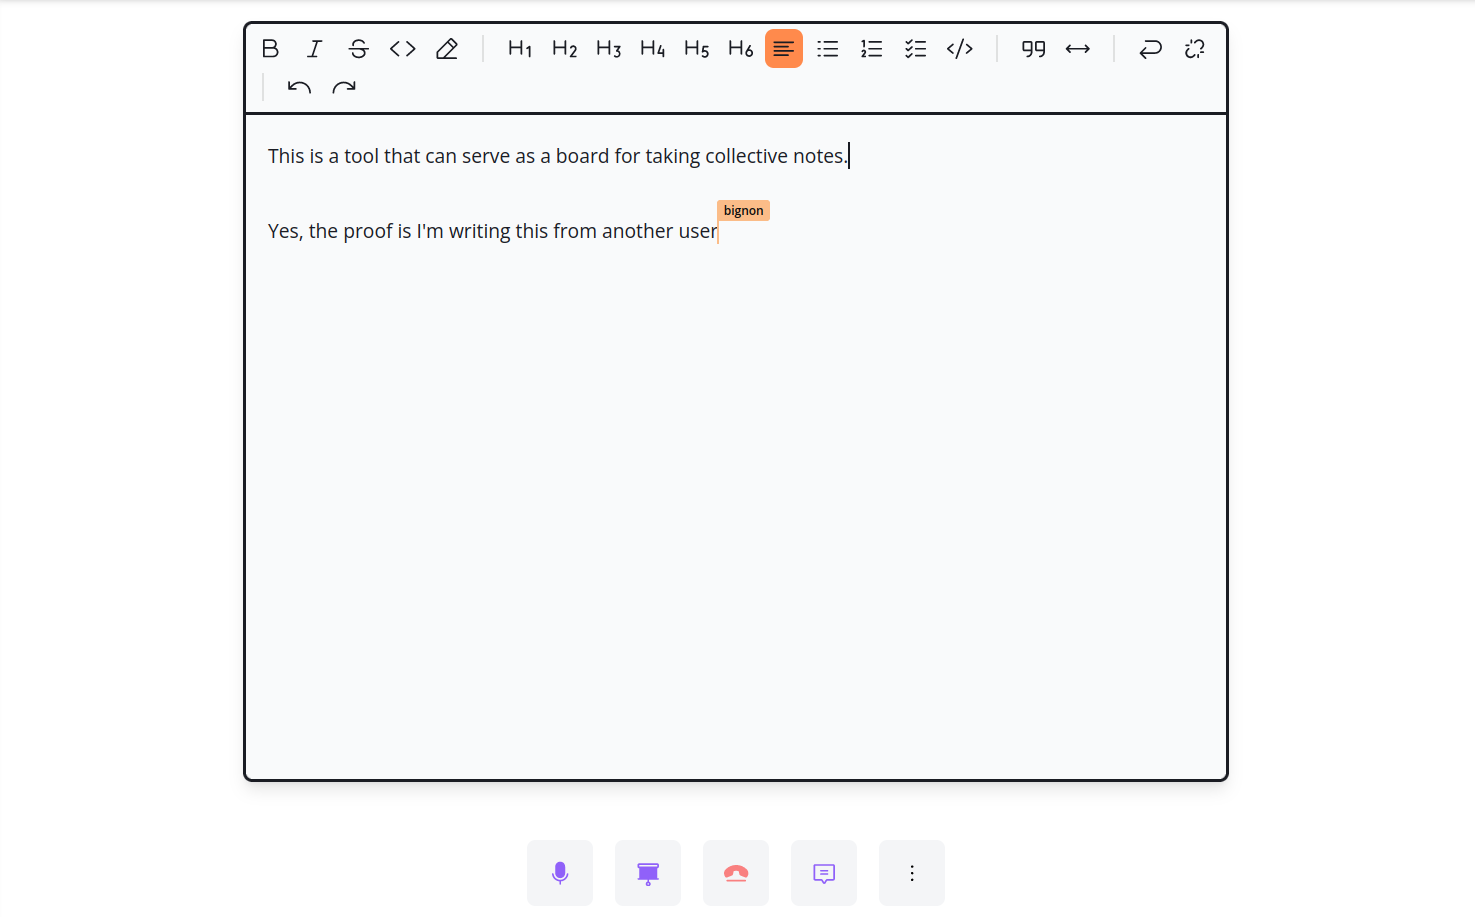
\includegraphics[width=0.85\textwidth]{prototype/wrritepad}}
  \caption{Outil de note synchronisé}
  \label{fig:writepad}
\end{figure}

Les fonctions suscitées rendent inaccessible la grille des participants. 
Mais il est toujours possible de pourvoir y accéder dans la même section que la messagerie, comme le montre la figure \ref{fig:participants_aside}.

\newpage
\begin{figure}[h]
  \centering
  \frame{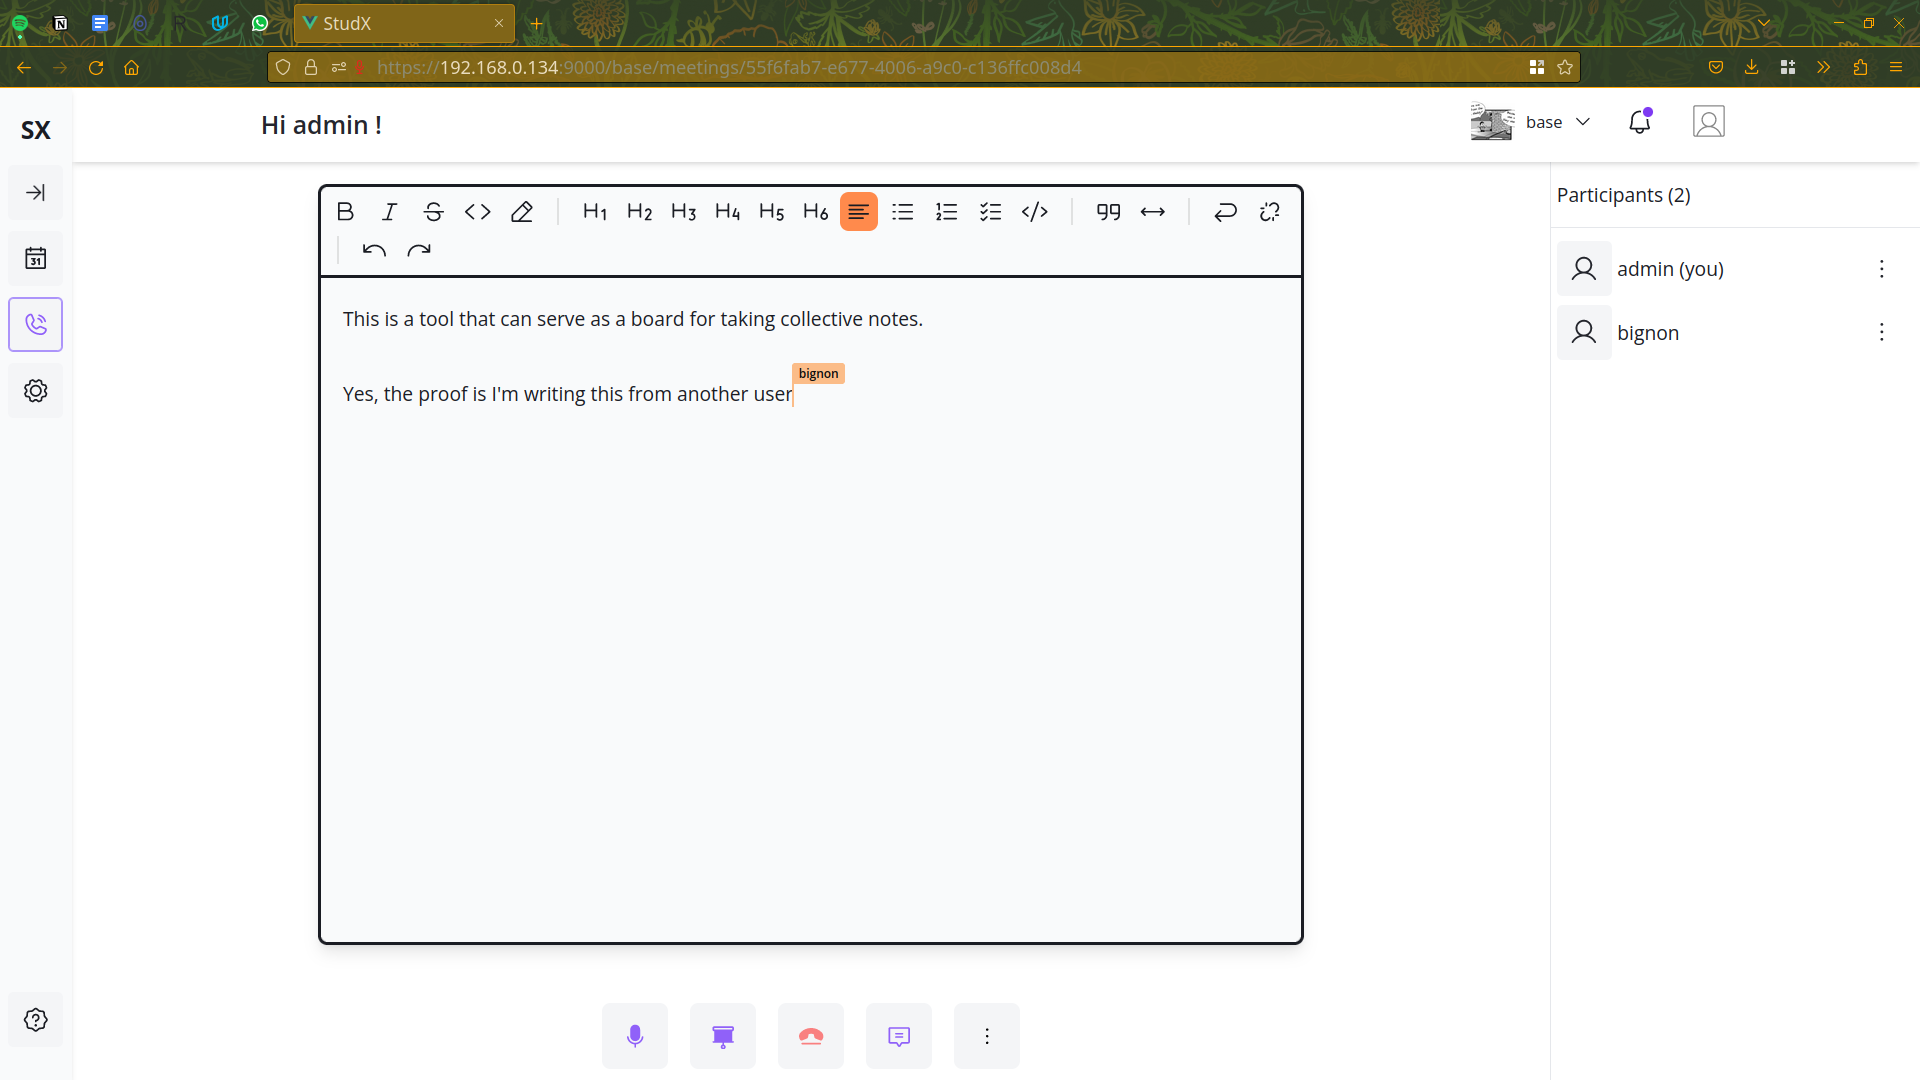
\includegraphics[width=0.85\textwidth]{prototype/participants}}
  \caption{Liste des participants}
  \label{fig:participants_aside}
\end{figure}

Enfin, chaque utilisateur a la possibilité de quitter la réunion. Si par mégarde, il essaie de recharger par exemple, l’onglet, une confirmation est requise (si le navigateur supporte cette fonctionnalité). 
Les figures \ref{fig:confirm_exit} et \ref{fig:exited} en font l'illustration.

\newpage
\begin{figure}[h]
  \centering
  \frame{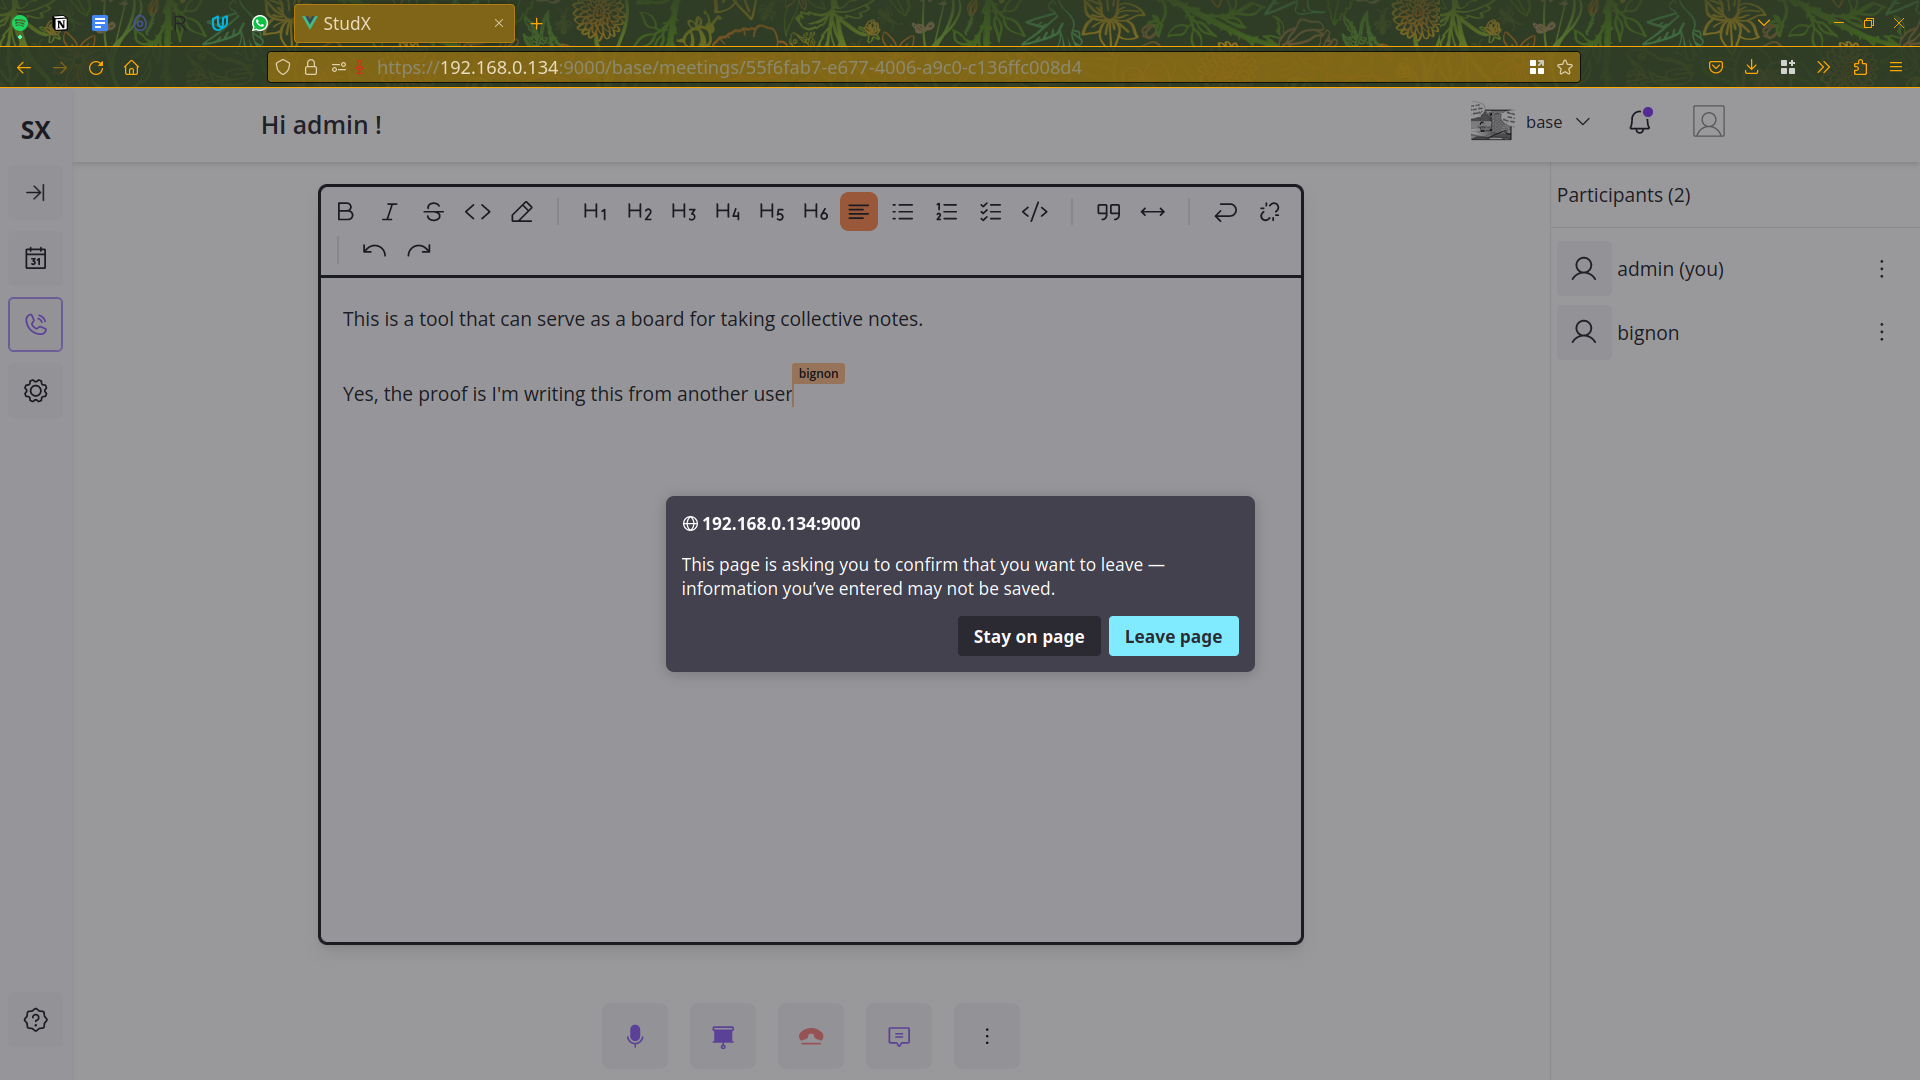
\includegraphics[width=0.85\textwidth]{prototype/confirm-exit}}
  \caption{Confirmation de déconnexion}
  \label{fig:confirm_exit}
\end{figure}

\begin{figure}[h]
  \centering
  \frame{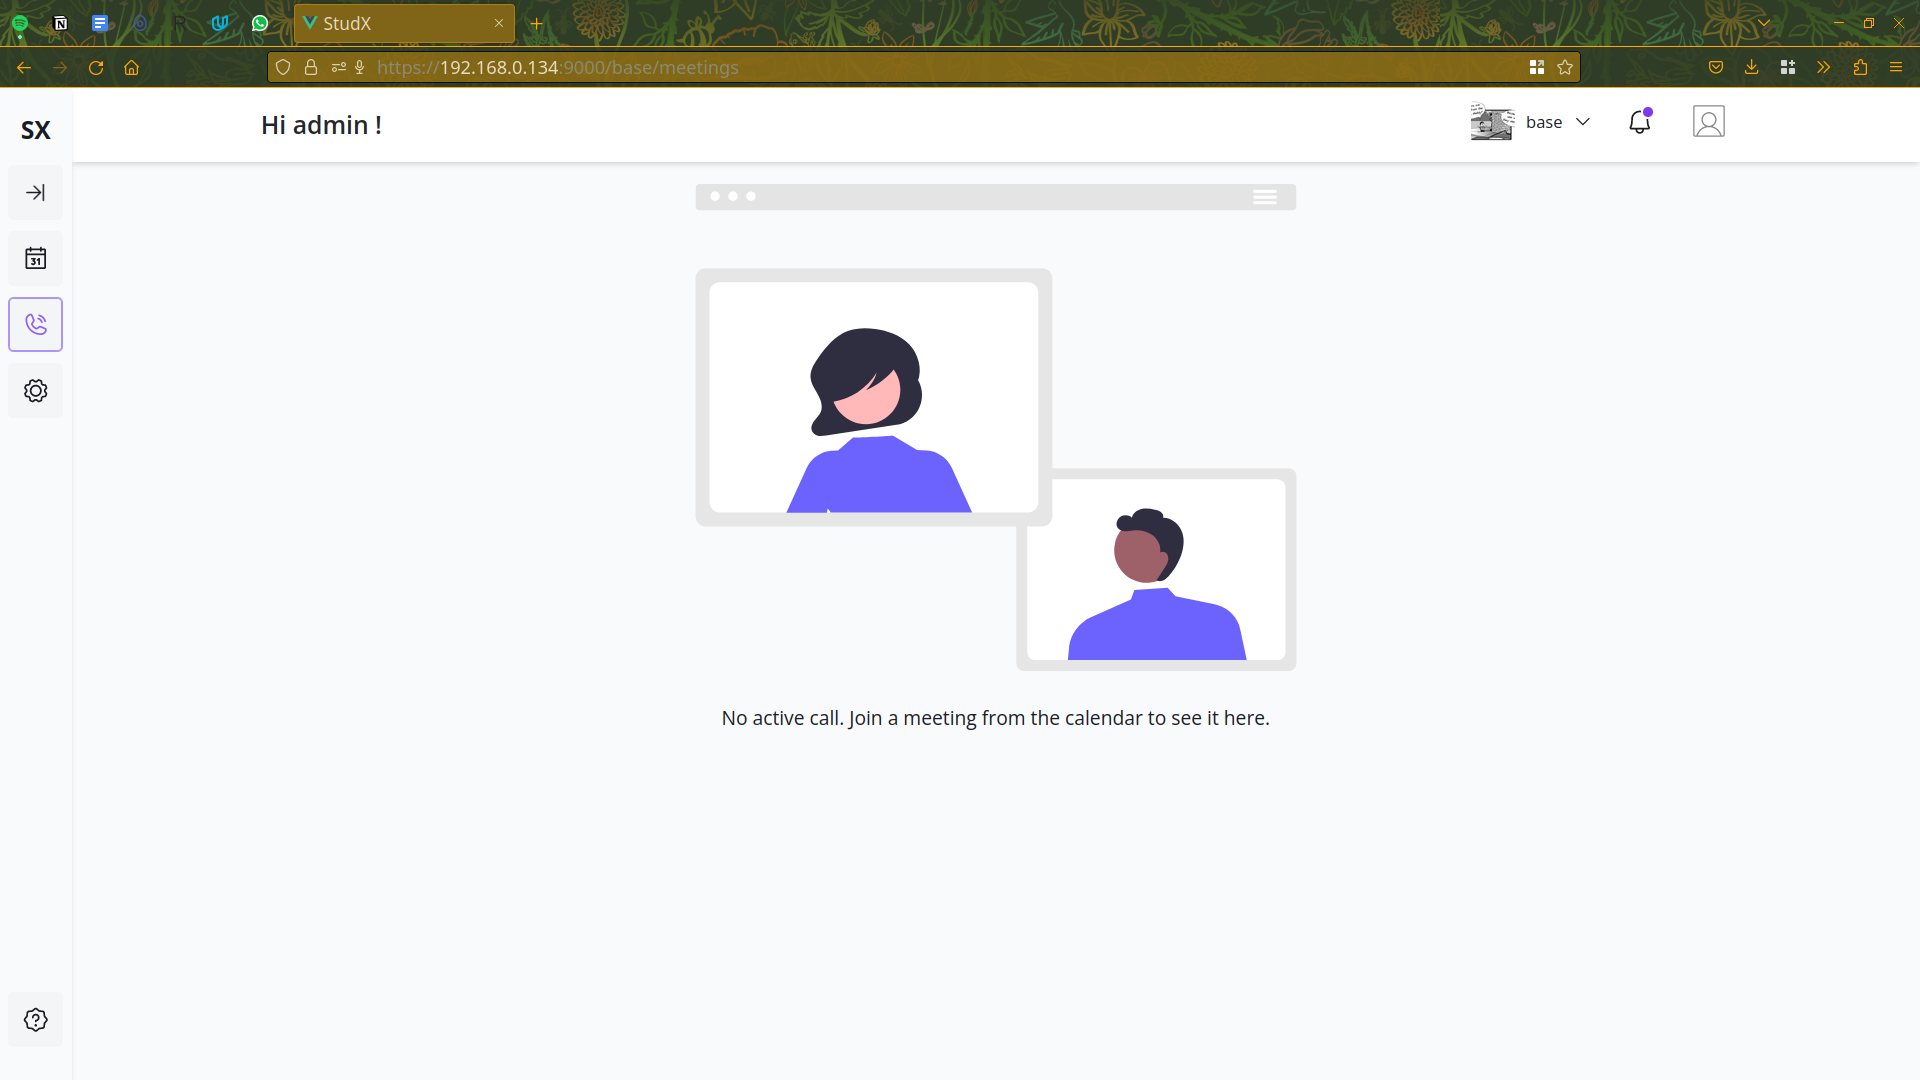
\includegraphics[width=0.85\textwidth]{prototype/no-active-call}}
  \caption{Page de redirection après déconnexion}
  \label{fig:exited}
\end{figure}

\subsection{Autres fonctionnalités}
Dans le but d'améliorer l'expérience utilisateur, nous avons jugé utile d’ajouter quelques fonctionnalités outre celles initialement visées. 
Parmi elles figurent le mode sombre et la mise en place d’un tutoriel interactif expliquant les diverses composantes de notre application. 

\newpage
\begin{figure}[h]
  \centering
  \frame{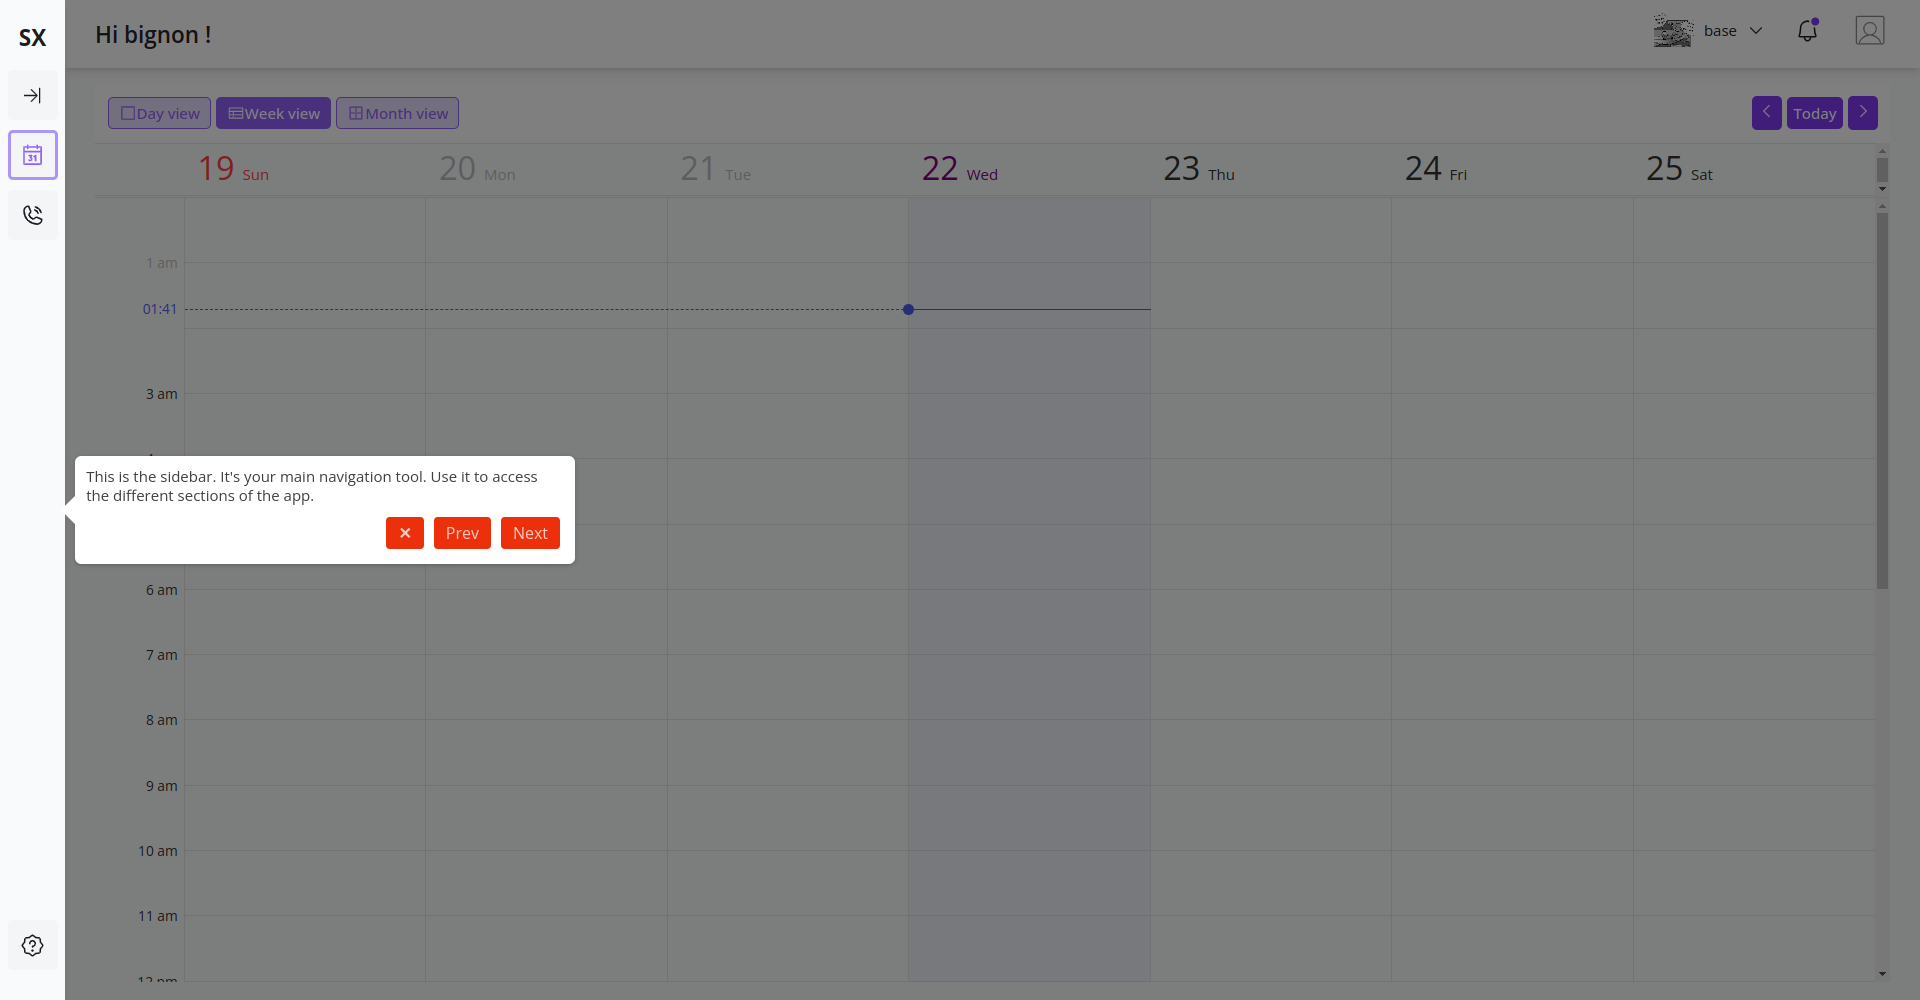
\includegraphics[width=0.85\textwidth]{prototype/user-onboarding}}
  \caption{Tutoriel interactif d’introduction à StudX}
  \label{fig:onboarding}
\end{figure}


\begin{figure}[h]
  \centering
  \frame{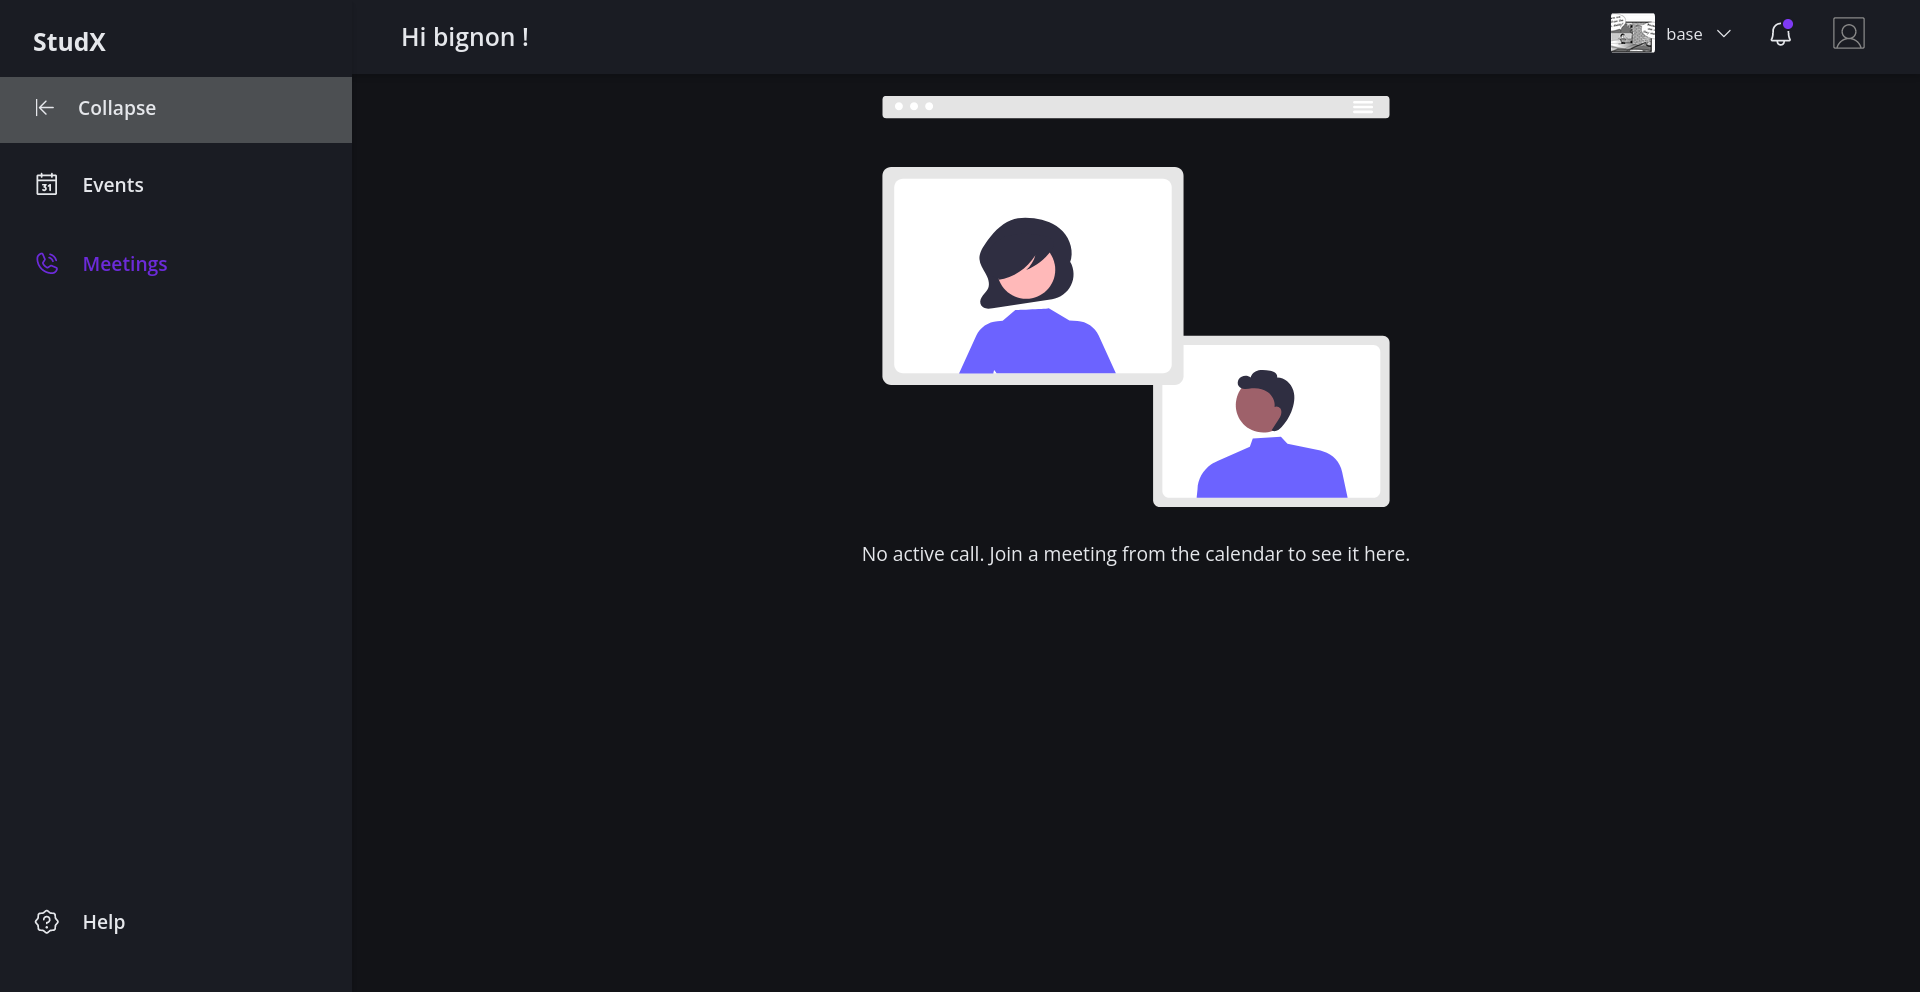
\includegraphics[width=0.85\textwidth]{prototype/wip-dark-mode}}
  \caption{Mode sombre}
  \label{fig:dark_mode}
\end{figure}

Les administrateurs de la plateforme disposent également d’un accès aux paramètres de 
l'organisation qu’ils dirigent et peuvent ainsi ajouter ou retirer des membres (figures \ref{fig:settings_one} et \ref{fig:settings_two}).

\begin{figure}[h]
  \centering
  \frame{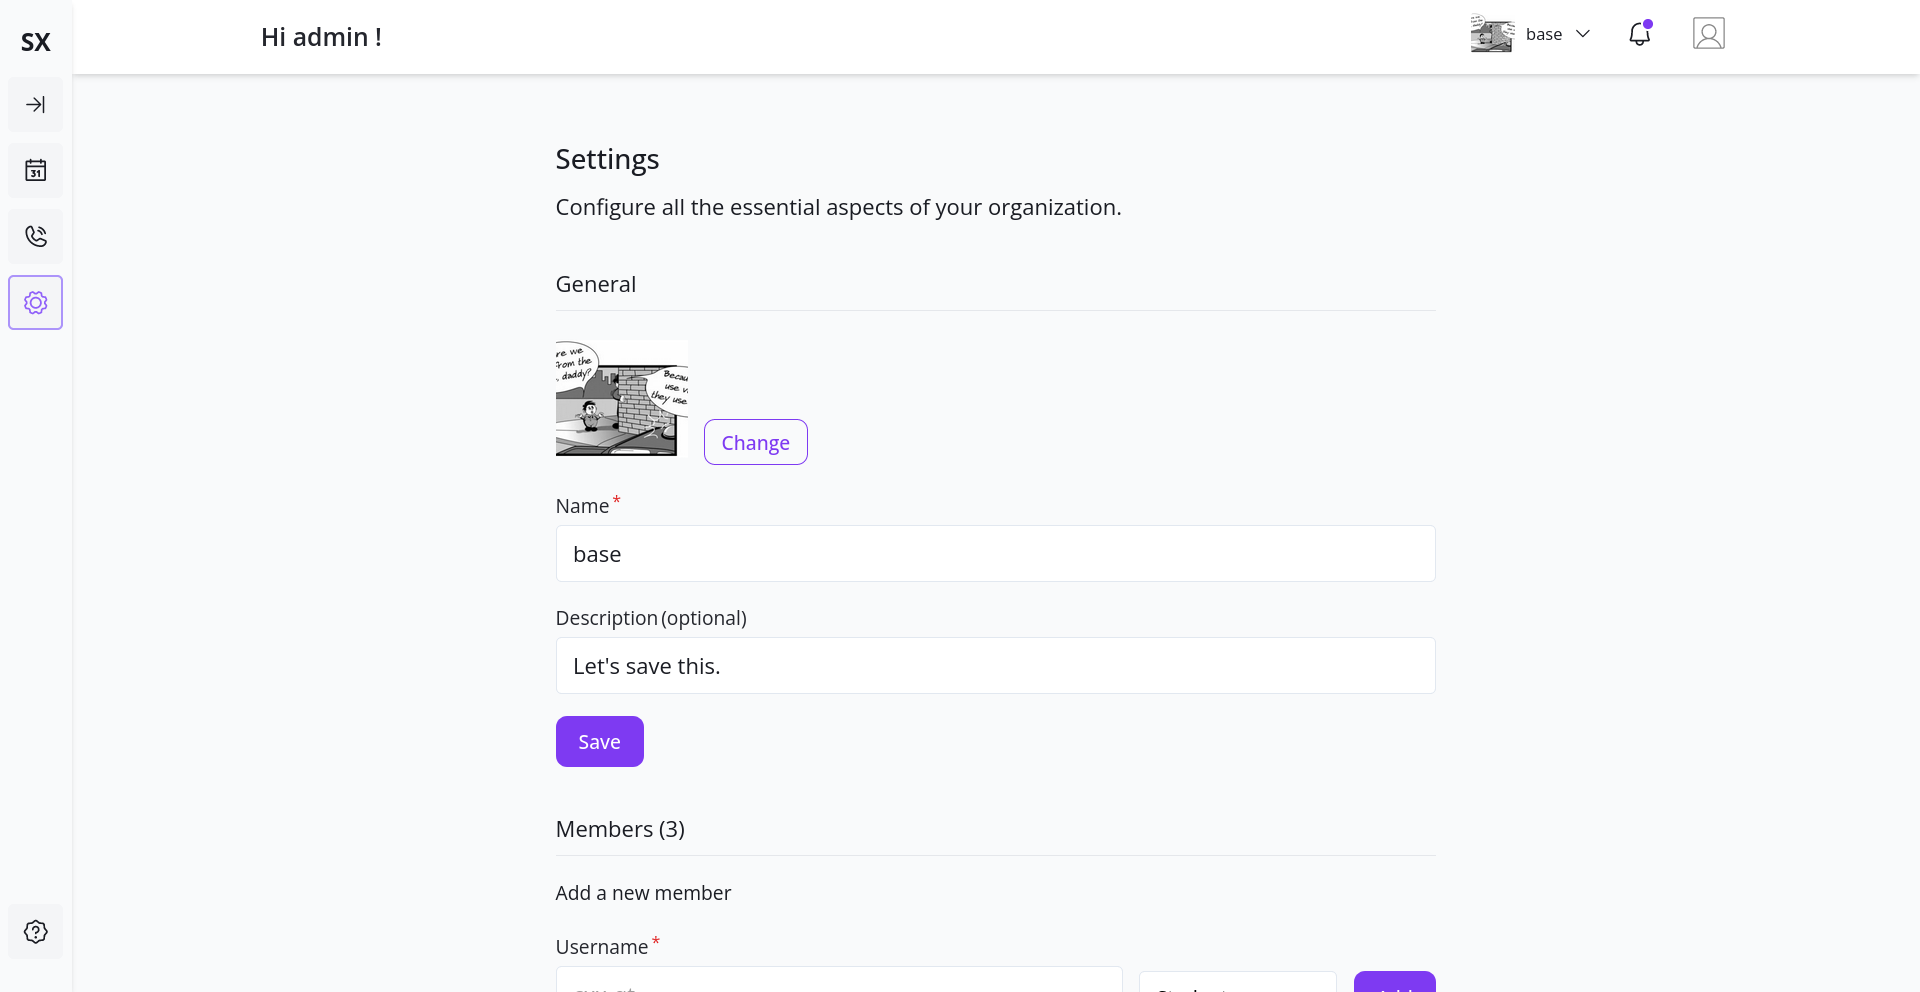
\includegraphics[width=0.85\textwidth]{prototype/settings}}
  \caption{Mode sombre}
  \label{fig:settings_one}
\end{figure}

\begin{figure}[h]
  \centering
  \frame{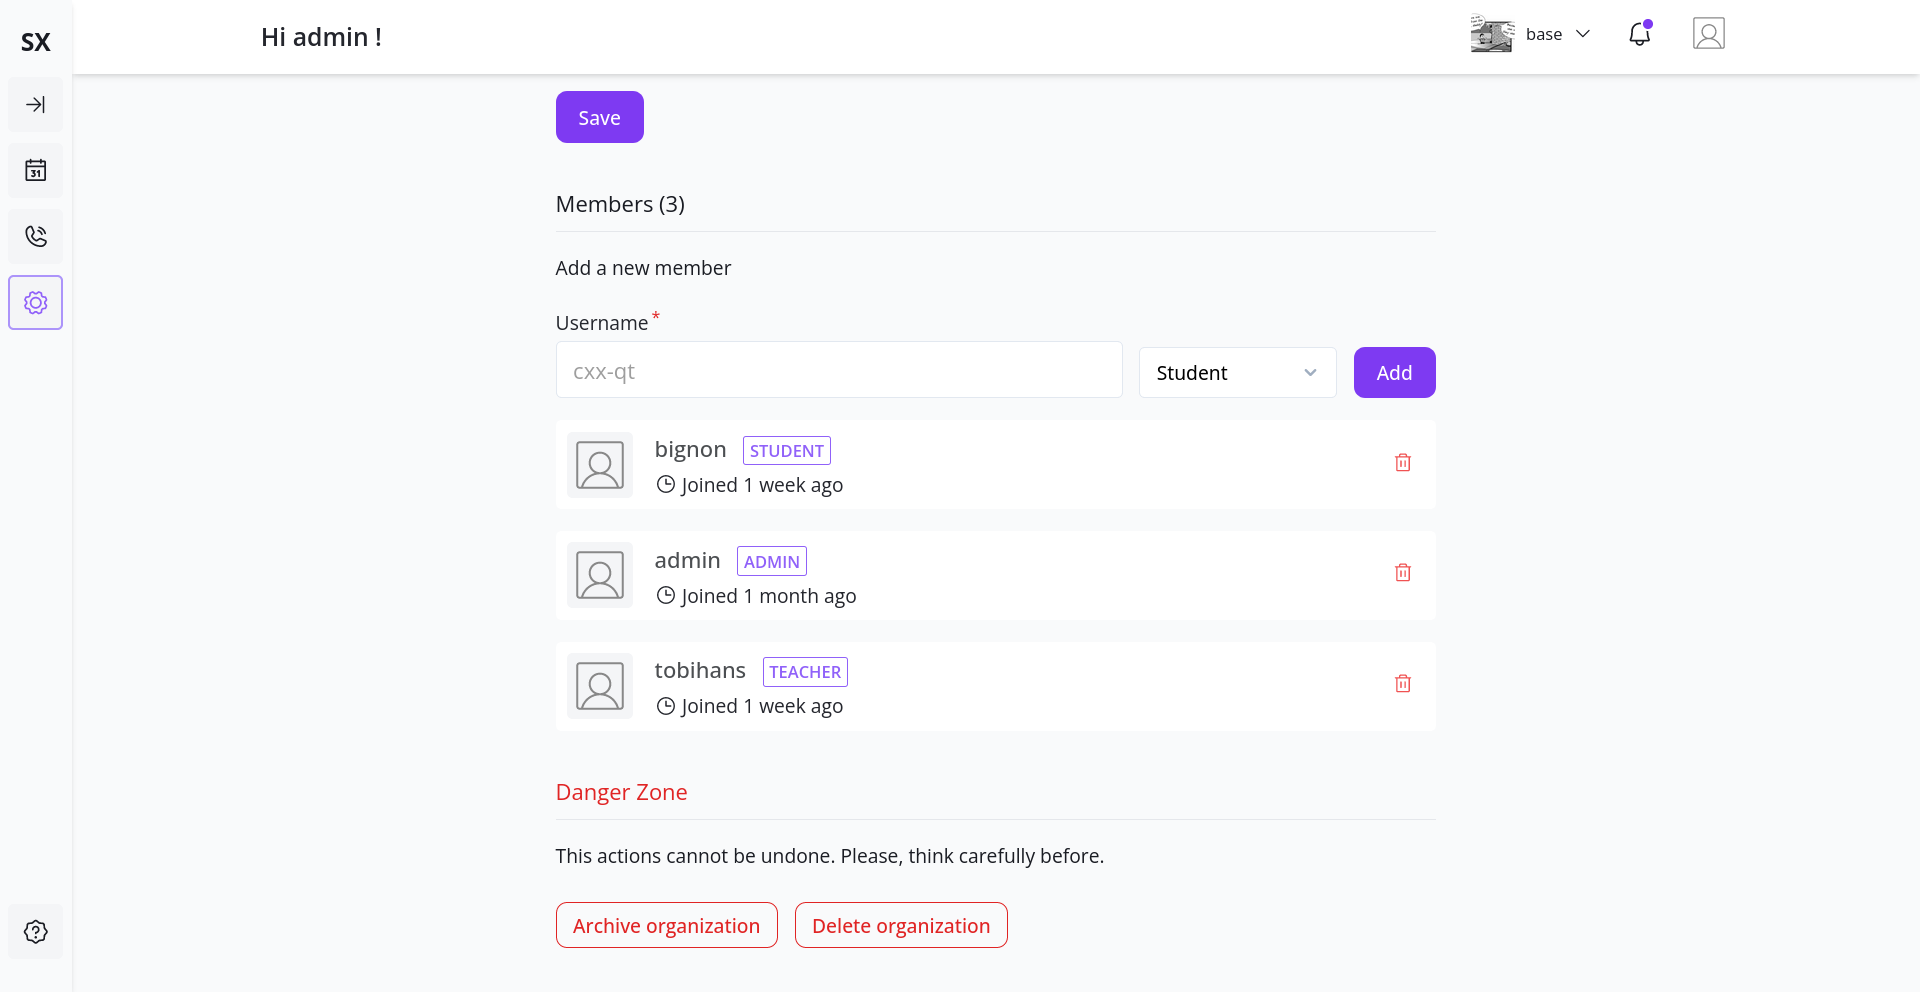
\includegraphics[width=0.85\textwidth]{prototype/settings-end}}
  \caption{Mode sombre}
  \label{fig:settings_two}
\end{figure}

\newpage
\section{Perspectives}
Le prototype StudX présente un ensemble de fonctionnalités utiles pour le déroulement de classes virtuelles. 
Toutefois, il présente certaines limites, outre les choix de conception comme l’absence de flux vidéo. 

En effet, la plateforme est conçue pour être accessible aux personnes disposant de toutes leurs facultés. 
Bien que les règles basiques d'accessibilité soient prises en compte, 
elles ne couvrent pas totalement le besoin. Par exemple, les personnes malentendantes 
n’ont pas la capacité de tirer profit des échanges vocaux qui sont effectués entre les divers participants. 
Une fonctionnalité envisagée est l'intégration de modèle de Machine Learning permettant la conversion de 
ces signaux audio en gestuelles dans le langage sourd.

Par ailleurs, dans le cadre d’un prototype, les fonctionnalités sont plutôt restreintes. 
On peut ajouter ou améliorer des fonctions comme la persistance de la messagerie instantanée ou 
encore la gestion des utilisateurs.


\addcontentsline{toc}{section}{Conclusion}
\section*{Conclusion}
Le prototype conçu répond à bien des besoins et couvre un tant soit peu l’ensemble des objectifs visés. 
Toutefois, il est possible de l’améliorer, dans le but d’en faire un plus large usage.